\clearpage
\section{Continuous Variable QKD Transmission System}\label{sec:intro}

\begin{tcolorbox}	
\begin{tabular}{p{2.75cm} p{0.2cm} p{10.5cm}} 	
\textbf{Student Name}  &:& Daniel Pereira (2017/05/01 - )\\
\textbf{Goal}          &:& Simulation and experimental validation of a CV-QKD transmission system.\\
\textbf{Directory}              &:& sdf/cv\_system  
\end{tabular}
\end{tcolorbox}

The aim of Continuous Variable Quantum Key Distribution (CV-QKD) is to encode information in observables whose measurements take continuous values.
\par
The purpose of this study is to analyse a CV-QKD transmission system in which the information is sent in the two orthogonal quadratures of a coherent state. 

\subsection{Theoretical Analysis}

The security of QKD is a complex topic to tackle, given the difficulty of proving the non-existence of an attack that cracks a protocol's security. This topic is usually approached by analysing various eavesdropping strategies and evaluating their effects on the key rate referenced in~\eqref{eq:keyrateperfect}. Information between Alice and Bob needs to be shared with current existing technology, so their shared information is always classical and Shannon's formalism is enough to describe it. However, Eve has no such restriction, so the information she has on Bob's results needs to be described according to the quantum properties of the system. 

\subsection{Simulation Analysis}

\begin{figure}[h]
\centering
%left bottom right top
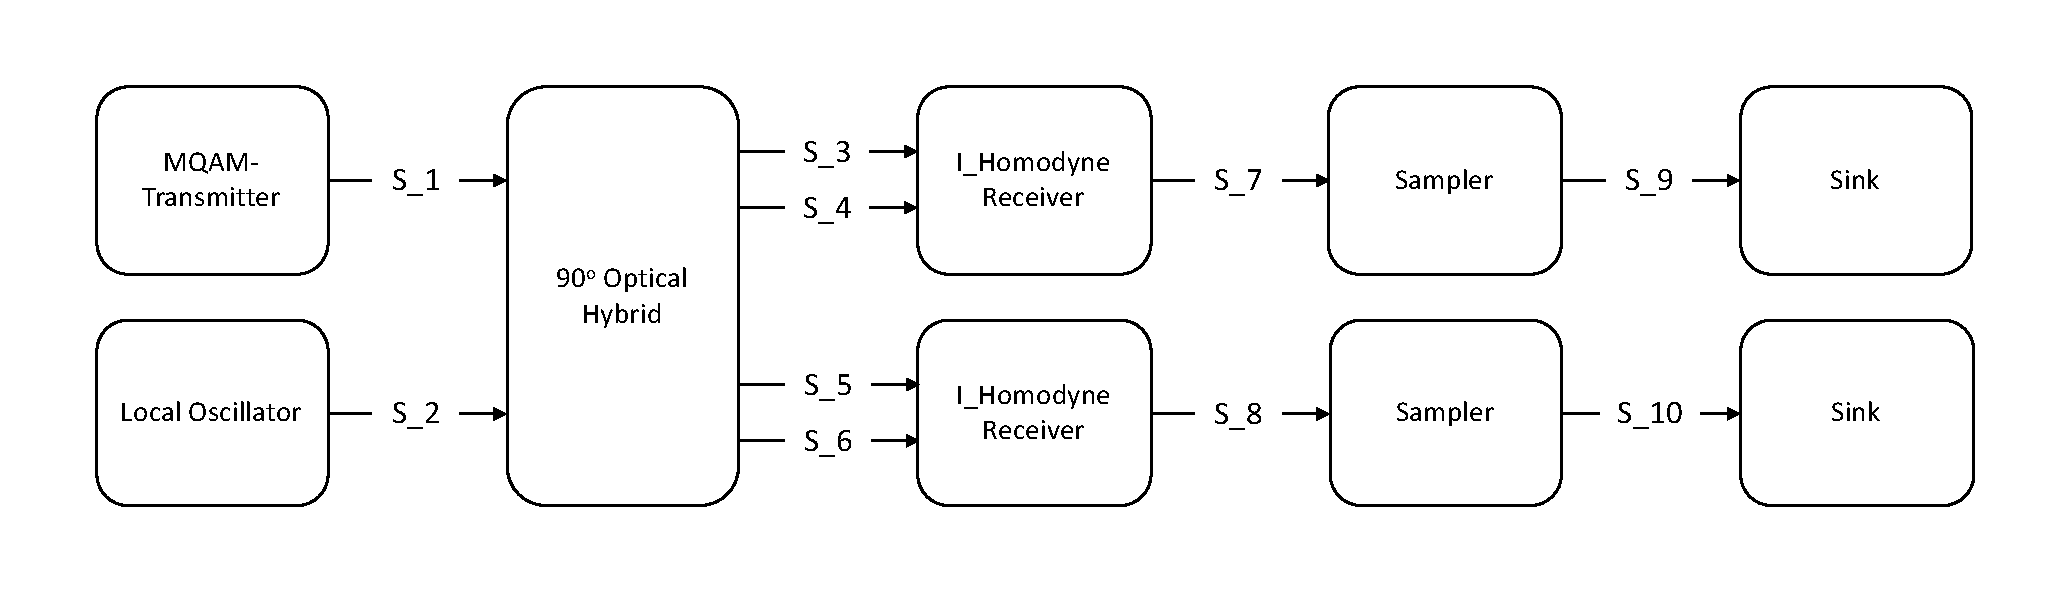
\includegraphics[width=\linewidth]{diagramSIMU.pdf}
\caption{Overview of the CV-QKD system being simulated.}
\label{fig:CV-System}
\end{figure}

\subsection*{Required files}\label{Required files}

\begin{table}[H]
\centering
\begin{tabulary}{1.0\textwidth}{|p{6cm}|p{8cm}|p{1cm}|}
\hline
\multicolumn{3}{|c|}{ \textbf{Header Files} } \\
\hline
\textbf{File}                    & \textbf{Comments} & \textbf{Status} \\ \hline
add.h                            &                   & \checkmark \\ \hline
binary\_source.h                 &                   & \checkmark \\ \hline
discrete\_to\_continuous\_time.h &                   & \checkmark \\ \hline
i\_homodyne\_reciever.h          &                   & \checkmark \\ \hline
ideal\_amplififer.h              &                   & \checkmark \\ \hline
iq\_modulator.h                  &                   & \checkmark \\ \hline
local\_oscillator.h              &                   & \checkmark \\ \hline
m\_qam\_mapper.h                 &                   & \checkmark \\ \hline
m\_qam\_transmitter.h            &                   & \checkmark \\ \hline
netxpto.h                        &                   & \checkmark \\ \hline
optical\_hybrid.h                &                   & \checkmark \\ \hline
photodiode.h                     &                   & \checkmark \\ \hline
pulse\_shaper.h                  &                   & \checkmark \\ \hline
sampler.h                        &                   & \checkmark \\ \hline
sink.h                           &                   & \checkmark \\ \hline
super\_block\_interface.h        &                   & \checkmark \\ \hline
white\_noise.h                   &                   & \checkmark \\ \hline
\end{tabulary}
\end{table}		
%
\begin{table}[H]
\centering
\begin{tabulary}{1.0\textwidth}{|p{6cm}|p{8cm}|p{1cm}|}
\hline
\multicolumn{3}{|c|}{ \textbf{Source Files} } \\
\hline
\textbf{File}                      & \textbf{Comments} & \textbf{Status} \\ \hline
add.cpp                            &                   & \checkmark \\ \hline
binary\_source.cpp                 &                   & \checkmark \\ \hline
discrete\_to\_continuous\_time.cpp &                   & \checkmark \\ \hline
i\_homodyne\_reciever.cpp          &                   & \checkmark \\ \hline
ideal\_amplififer.cpp              &                   & \checkmark \\ \hline
iq\_modulator.cpp                  &                   & \checkmark \\ \hline
local\_oscillator.cpp              &                   & \checkmark \\ \hline
m\_qam\_mapper.cpp                 &                   & \checkmark \\ \hline
m\_qam\_transmitter.cpp            &                   & \checkmark \\ \hline
netxpto.cpp                        &                   & \checkmark \\ \hline
optical\_hybrid.cpp                &                   & \checkmark \\ \hline
photodiode.cpp                     &                   & \checkmark \\ \hline
pulse\_shaper.cpp                  &                   & \checkmark \\ \hline
sampler.cpp                        &                   & \checkmark \\ \hline
sink.cpp                           &                   & \checkmark \\ \hline
super\_block\_interface.cpp        &                   & \checkmark \\ \hline
white\_noise.cpp                   &                   & \checkmark \\ \hline
\end{tabulary}
\end{table}		

\subsection*{System Input Parameters}

This system takes into account the following input parameters:

\begin{table}[H]
\centering
\begin{tabulary}{1.0\textwidth}{|p{6cm}|p{4cm}|p{5cm}|}
\hline
\multicolumn{3}{|c|}{ \textbf{System Input Parameters} } \\
\hline
\textbf{Parameter}     & \textbf{Default Value}                                     & \textbf{Comments} \\ \hline
numberOfBitsGenerated  & $40000$	                                                   &                     \\ \hline
bitPeriod              & $20\times10^{-12}$                                         &\\ \hline
samplesPerSymbol       & $16$                                                       &\\ \hline
pLength                & $5$                                                        &\\ \hline
iqAmplitudesValues     & $\lbrace~\lbrace-1,~0\rbrace~,~\lbrace1,~0\rbrace~\rbrace$ & \\ \hline
outOpticalPower\_dBm   & Variable                                                   & Value varied for presented study\\ \hline
loOutOpticalPower\_dBm & $0$                                                        & \\ \hline
localOscillatorPhase   & $0$                                                        & \\ \hline
transferMatrix         & $\lbrace~\lbrace \frac{1}{\sqrt{2}},~\frac{1}{\sqrt{2}},~\frac{1}{\sqrt{2}},~\frac{-1}{\sqrt{2}} \rbrace~\rbrace$ & \\ \hline
responsivity           & $1$                                                        & \\ \hline
amplification          & $10^3$                                                     & \\ \hline
noiseSpectralDensity   & $5\times10^{-4}\sqrt{2}$~V$^2$                             & \\ \hline
confidence             & $0.95$                                                     & \\ \hline
midReportSize          & $0$                                                        & \\ \hline
\end{tabulary}
\end{table}		

\subsection*{Inputs}

This system takes no inputs.

\subsection*{Outputs}

This system outputs the following objects:
\begin{itemize}
\item Signals:
\begin{itemize}
\item Optical Signal with coded Binary String; (S$_{1}$)
\item Local Oscillator Optical Signal; (S$_{2}$)
\item 90$^\text{o}$ Optical Hybrid Outputs; (S$_{3}$, S$_{4}$, S$_{5}$, S$_{6}$)
\item Homodyne Detectors' Electrical Output; (S$_{7}$, S$_{8}$)
\item Sampled Signals; (S$_{9}$, S$_{10}$)
\end{itemize}
\end{itemize}


\subsection{Experimental Analysis}

The main experimental setup used is presented in Figure~\ref{fig:expDia}.
\begin{figure}[H]
\centering
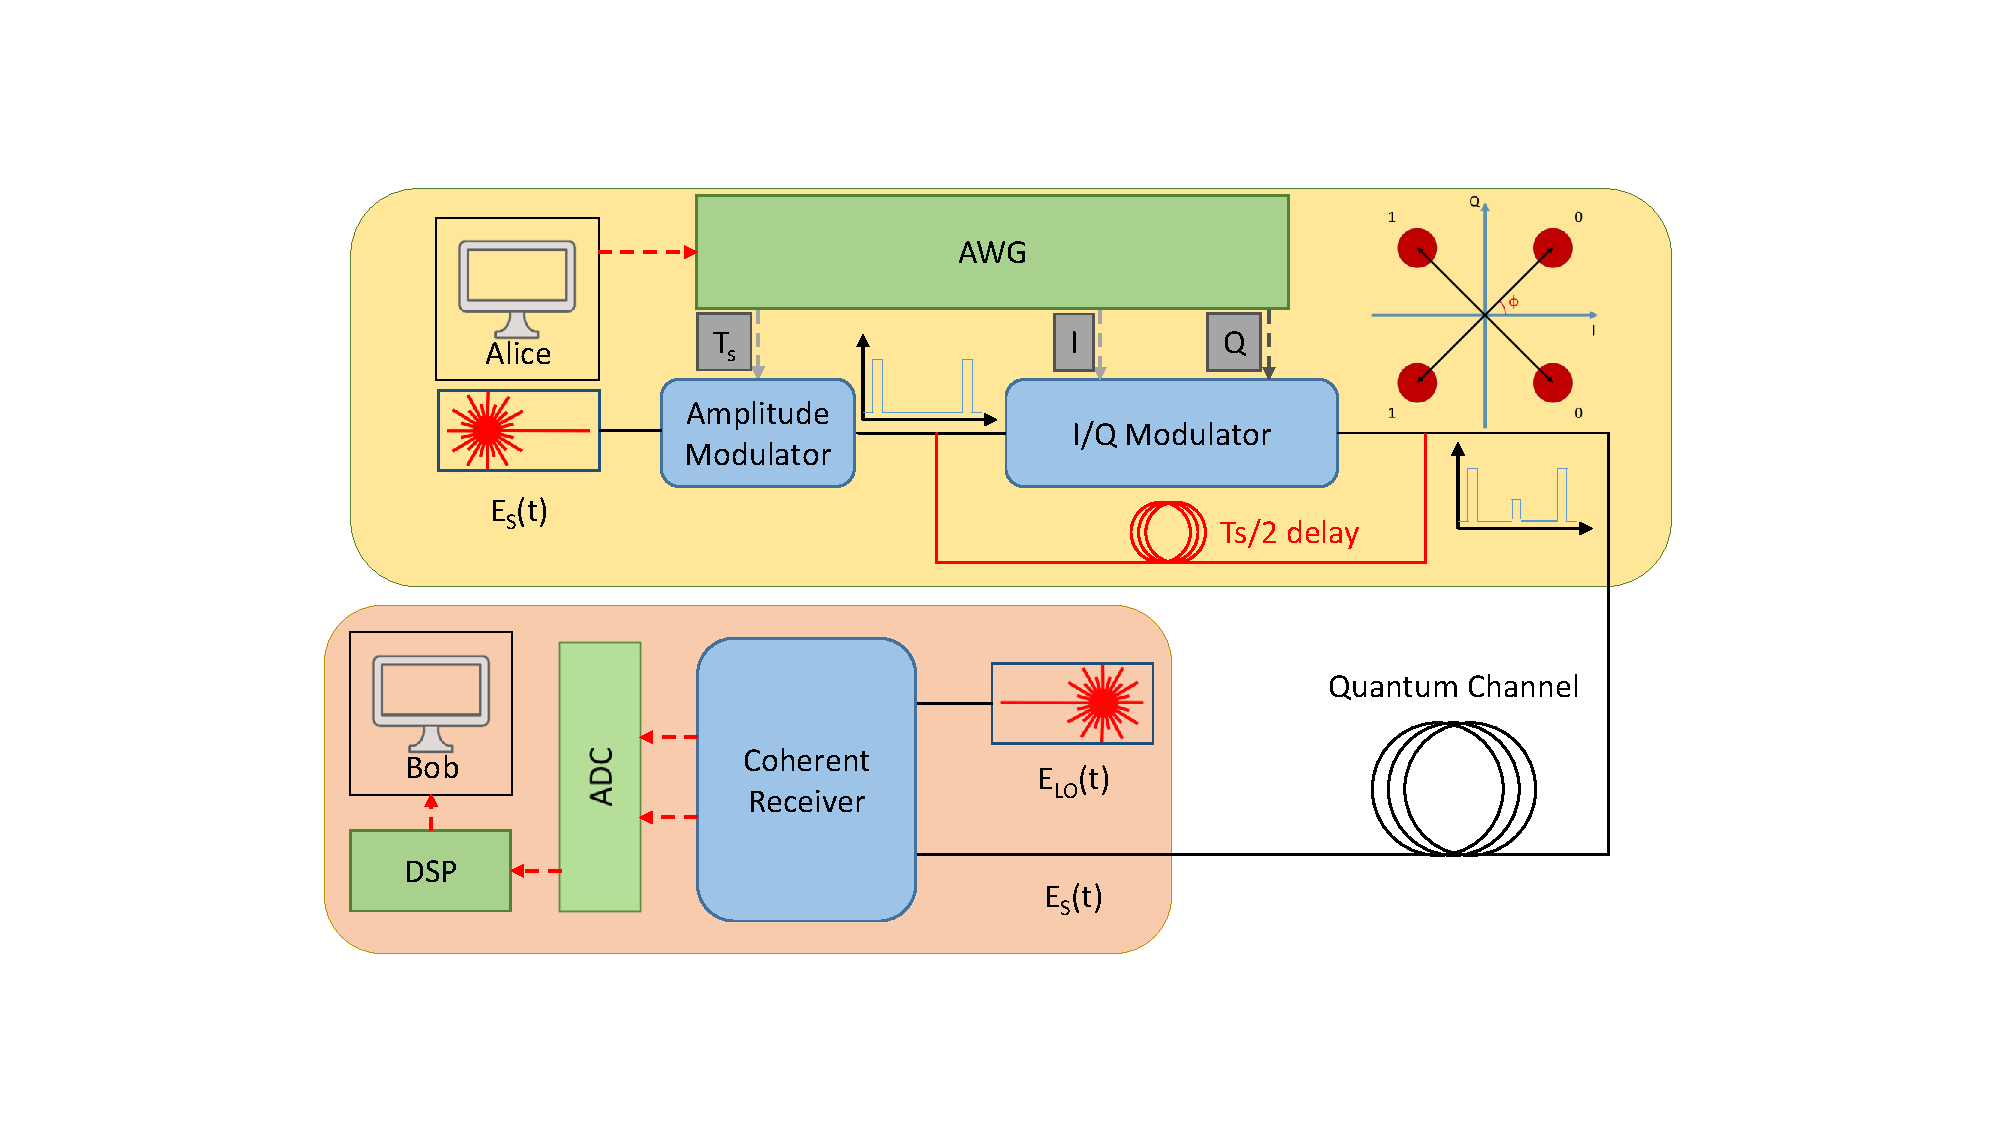
\includegraphics[width=\linewidth, trim={0cm 2.5cm 0cm 3cm}, clip=true]{withtrace.pdf}
\caption{Diagram of full experimental setup.}
\label{fig:expDia}
\end{figure}
The setup contained two Yenista OSICS Band C/AG TLS lasers, tuned to a 1550~nm wavelength. A JDSU dual drive Mach-Zehnder Modulator with a Picosecond 5865 RF driver, employed at the output of one of the lasers and acting as an amplitude modulator, set the repetition rate at 1~GHz with a pulse time of 125~ps. This amplitude modulated laser is dubbed the Signal (\textbf{SI}) laser. The driving signal was generated by an Agilent Technologies BER Tester. A 50/50 beam-splitter was employed at the output of the Mach-Zehnder Modulator, one arm output is sent through an IQ Modulator while the other is sent through a fibre loop with length chosen such that the two arms have a relative delay of roughly 500~ps. The employed IQ Modulator was a u2t Photonics 32~GHz IQ Modulator with a SHF 807 RF driver, the driving signal being generated by a Tektronix AWG70002A Arbitrary Waveform Generator (\textbf{AWG}). A 15~dB attenuator followed by a Variable Optical Attenuator (\textbf{VOA}) was set at the output of the IQ modulator to allow a fine tuning of the phase modulated signal's optical power to the desired level. The two arms created by the first beam-splitter are combined by a 50/50 beam combiner. A fibre channel of $\sim10$~km was set between Alice's and Bob's setup. The second Yenista OSICS Band C/AG TLS laser, from this point dubbed the Local Oscillator (\textbf{LO}) laser, was sent through a VOA to a coherent receiver. A Picometrix CR-100D 100G Integrated Balanced Receiver for Coherent Applications with a bandwidth of  30~GHz was employed to perform double homodyne measurements, recovering both the in-phase and in-quadrature components of the incoming light field. The response of the receiver was recorded by a Tektronix DPO77002SX-R3 oscilloscope, with an acquisition frequency of 100~GHz for a period of 400~\textmu{s}.
\par
Some variations of the setup presented in Figure~\ref{fig:expDia} were used, for example using one laser instead of the two presented (adding a 50/50 beamsplitter before the Mach-Zehnder Modulator to extract the local oscillator from the same source as the signal), dubbed single laser setup, and removing the Quantum-Channel (connecting the signal generation setup directly to the detection), dubbed back to back setup. With these changes, a total of 4 setups were implemented. The objective of these changes was to reduce complexity and allow for easier identification and correction of possible errors in the experimental setup.
\par
The driving signal implemented on the AWG was generated by a short Matlab code that generated a Pseudo Random Bit Sequence (\textbf{PRBS}) with length $2^{17}$ preceded by a deterministic tram of length 32896 taking the form $1001110000(...)$.

\subsection{Comparative Analysis}

\bibliographystyle{unsrt}
 
\bibliography{bibliography}
